\documentclass{article}
\usepackage{url}
\usepackage{mathtools}
\usepackage{amsmath}
\usepackage{listings}
\usepackage{graphicx}
\usepackage[margin=1in]{geometry}
\lstset{breaklines=true}
\begin{document}

\title{CS595 Intro to Web Science, Assignment \#1}
\author{Valentina Neblitt-Jones}
\date{September 12, 2013}
\maketitle

\section{cURL Exercise}
\textbf {Demonstrate that you know how to use "curl" well enough to correctly POST data to a form.  Show that the HTML response that is returned is "correct" (e.g., save it to a file and then view that file in a browser and take a screen shot).}

Finding a web form that did not require me revealing my credentials and actually used the POST method was quite difficult. I used W3C Markup Validator Service \url{http://validator.w3.org/#validate_by_input}. It was being extra fussy about the special characters (--urlencode was not solving the problem) so so I had to substitute the appropriate URL encoding using \url{http://www.w3schools.com/tags/ref_urlencode.asp}. My cURL statement follows.

\begin{lstlisting}
curl --data "fragment=%3Cp%3ECurrently I am 40 years old and an academic systems librarian. My passions are books, movies, and television. My ultra-passions include Star Wars, LEGO, The Simpsons, and Harry Potter.%3C%2Fp%3E&prefill=1&doctype=Inline&fbd=1&prefill_doctype=html401&group=0&ss=1&st=1&outline=1&No200=1&verbose=1" --url http://validator.w3.org/check -o debug.html
\end{lstlisting}

The four screenshots below illustrate the difference in how the page was rendered when using the browser versus cURL to fill out the form. Figures 1 \& 2 show the browser version and Figures 3 \& 4 show the cURL version. Although the stylesheet and images are missing from the cURL version, the same information is present.

\begin{figure}
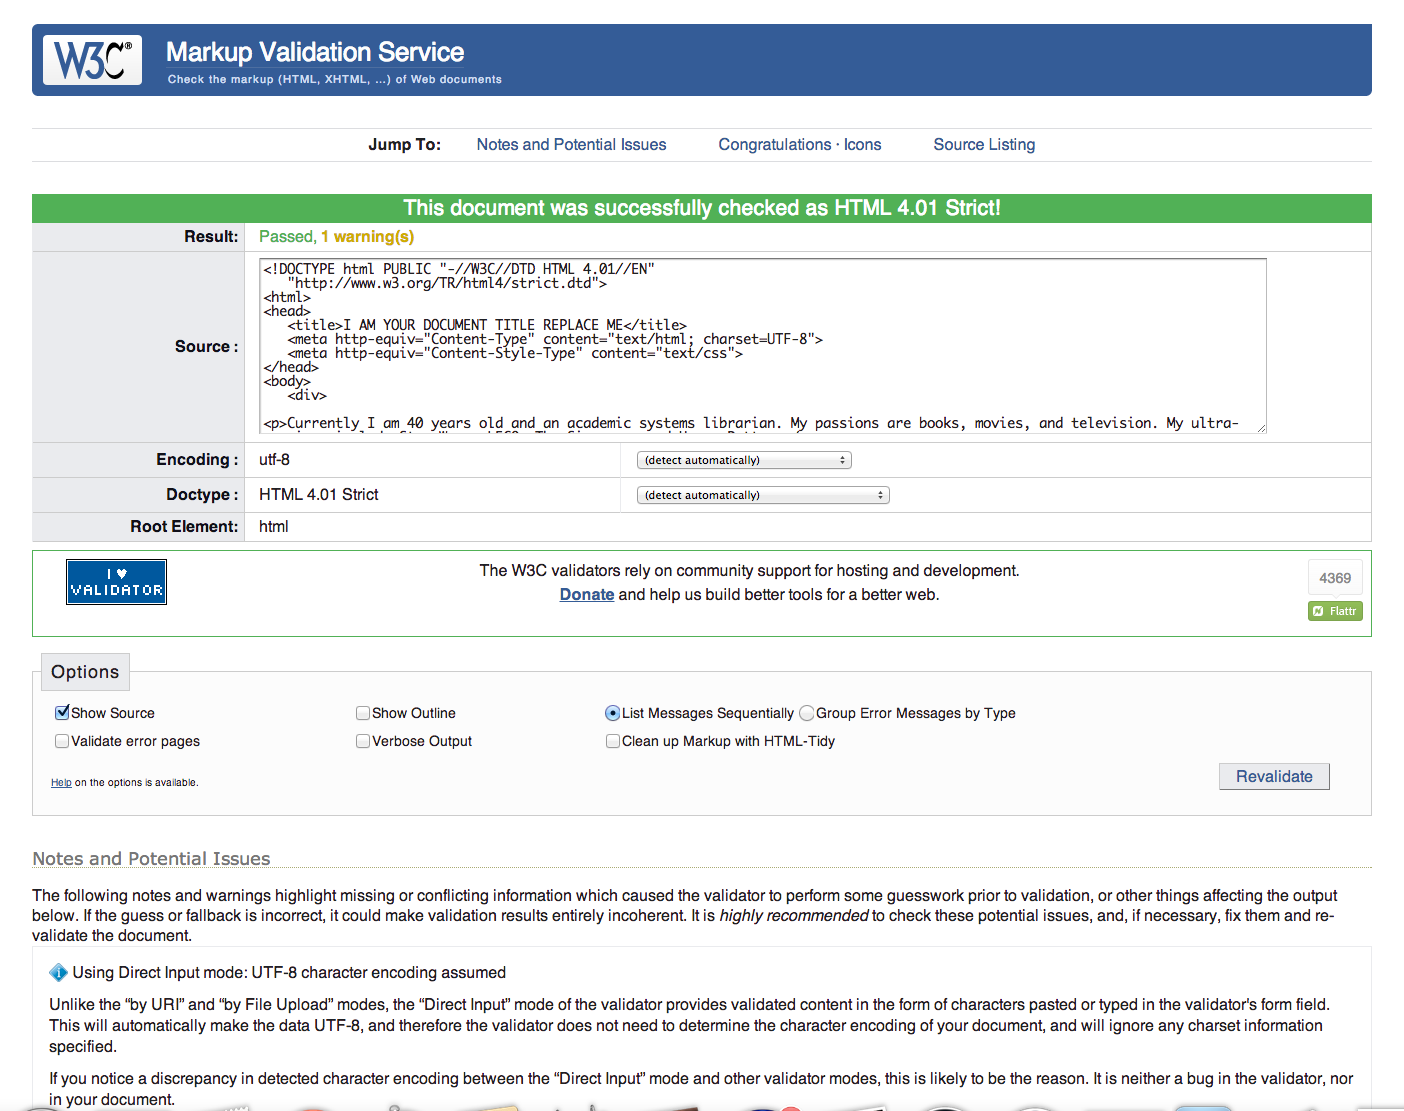
\includegraphics[scale=0.30]{w3cMarkupValidationServiceNormal01}
\caption{This is the top half of the screen representing output when the browser was used to fill out the form}
\end{figure}

\begin{figure}
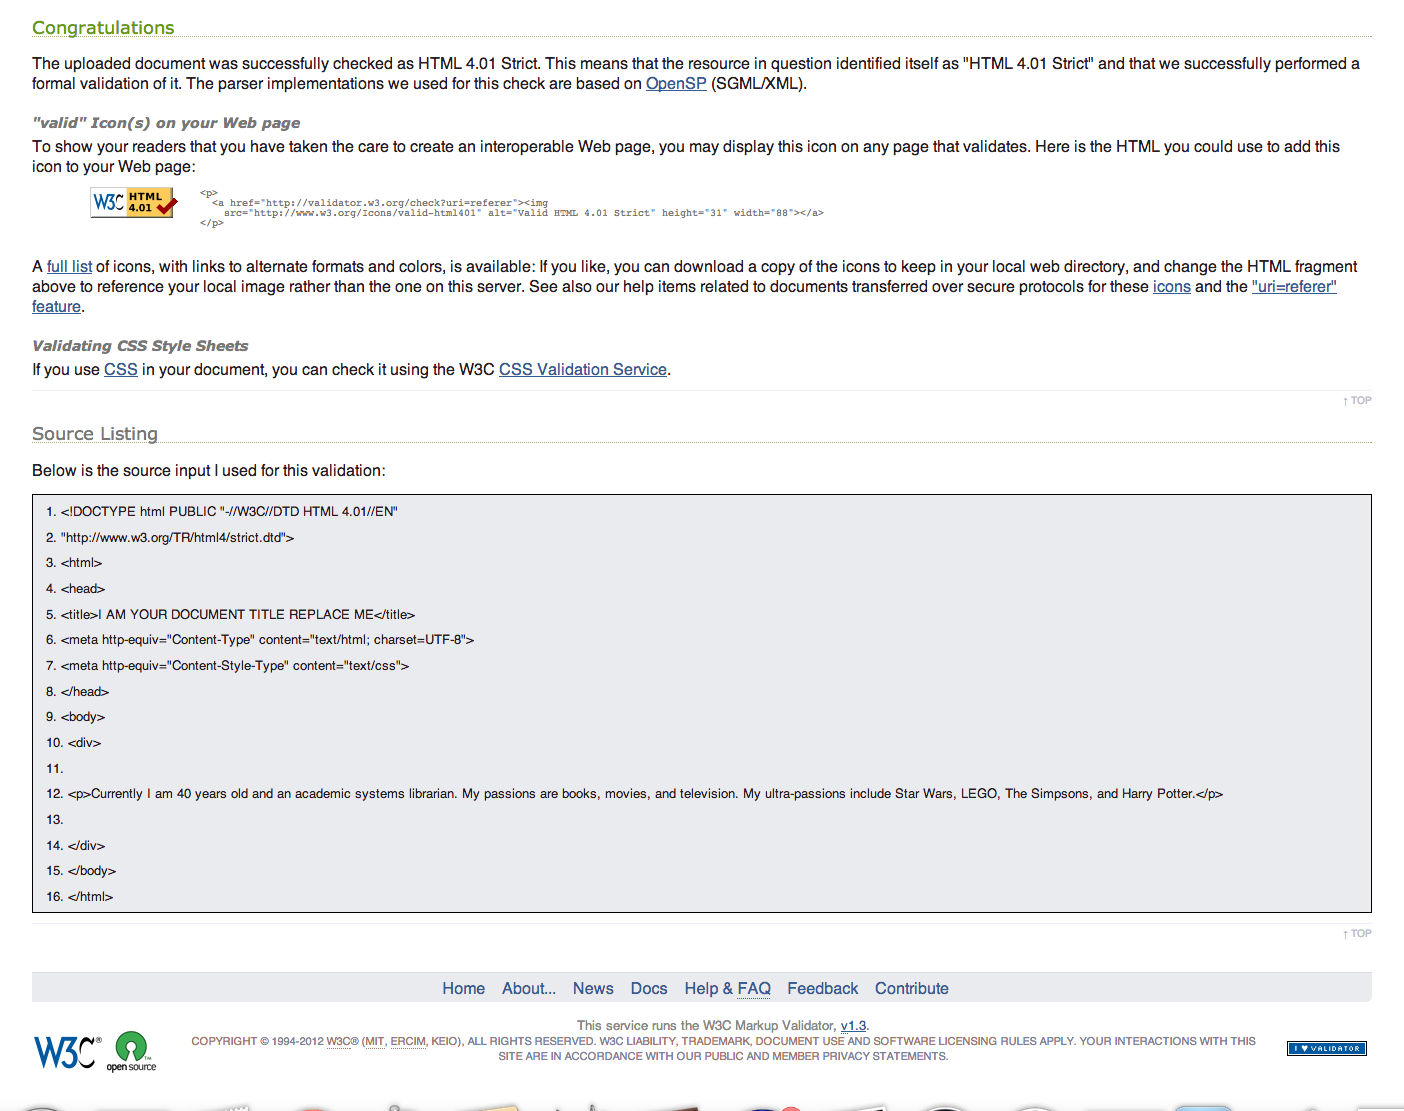
\includegraphics[scale=0.30]{w3cMarkupValidationServiceNormal02}
\caption{This is the bottom half of the screen representing output when the browser was used to fill out the form}
\end{figure}

\begin{figure}
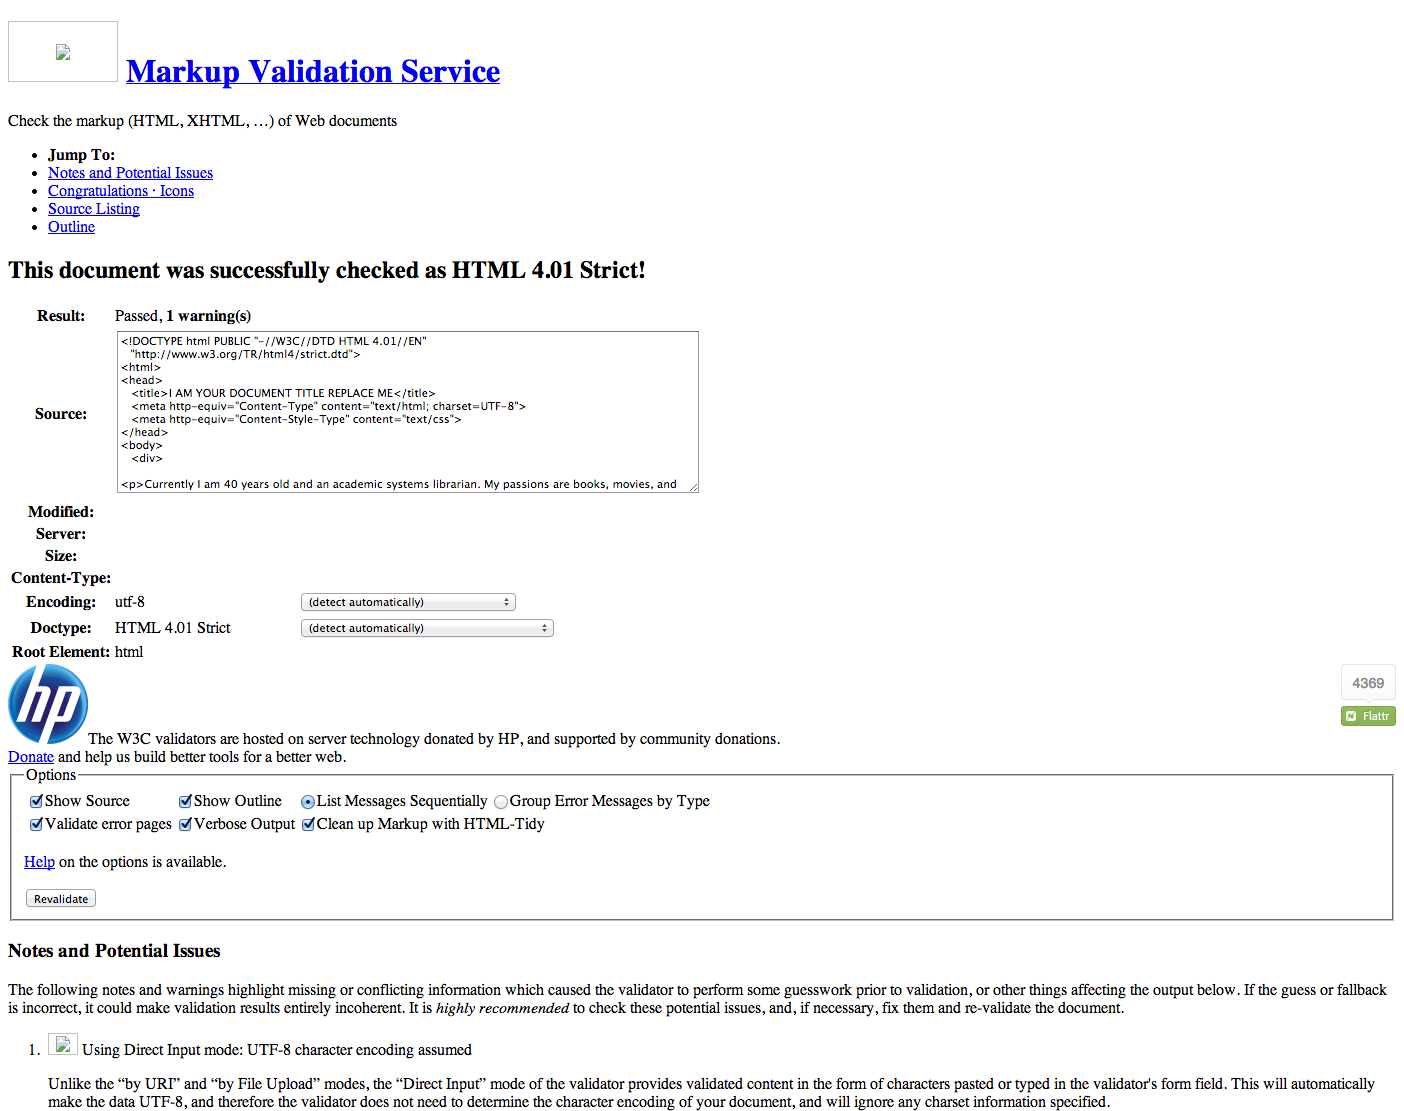
\includegraphics[scale=0.30]{w3cMarkupValidationServiceCurl01}
\caption{This is the top half of the screen representing output when cURL was used to fill out the form}
\end{figure}

\begin{figure}
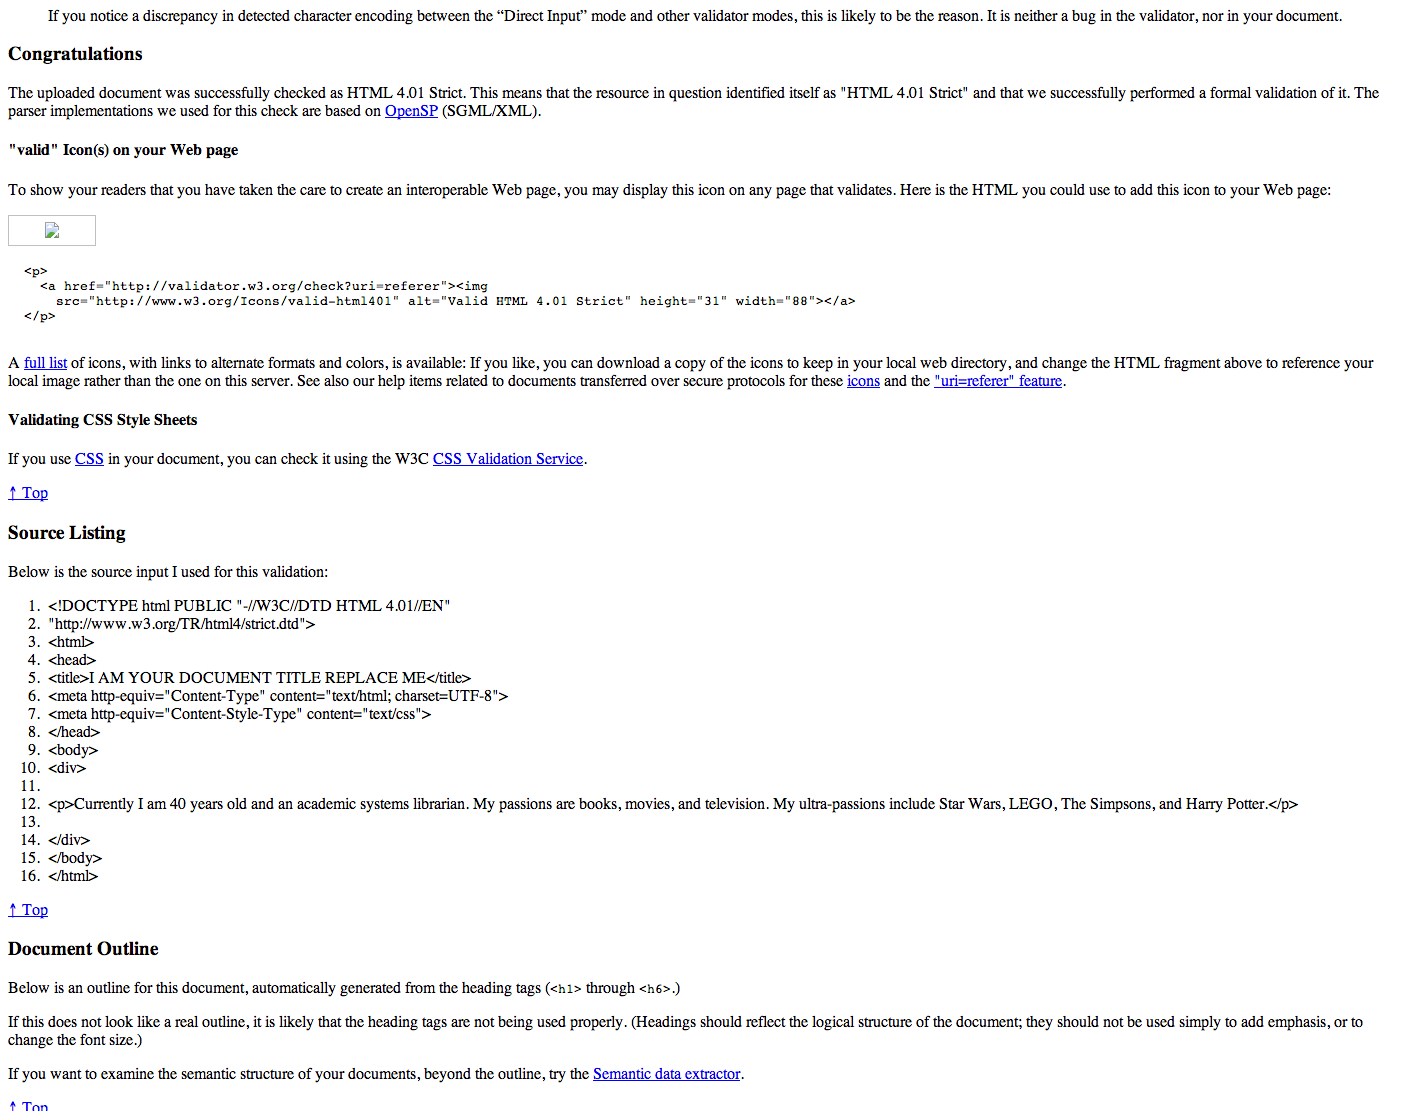
\includegraphics[scale=0.30]{w3cMarkupValidationServiceCurl02}
\caption{This is the bottom half of the screen representing output when cURL was used to fill out the form}
\end{figure}

\newpage

\section{Python Exercise}
\textbf{Write a Python program that:
(1)Takes one argument, like "Old Dominion" or "Virginia Tech" (2) takes another argument specified in seconds (e.g., "60" for one minute) (3) takes a URI as a third argument: \url{http://scores.espn.go.com/ncf/scoreboard?confId=80&seasonYear=2013&seasonType=2&weekNumber=2} \textbf{OR} \url{http://scores.espn.go.com/ncf/scoreboard?confId=80&seasonYear=2013&seasonType=2&weekNumber=1} \textbf{OR} \url{http://scores.espn.go.com/ncf/scoreboard?confId=80&seasonYear=2012&seasonType=2&weekNumber=1} etc. and (4) downloads the URI, finds the game corresponding to the team argument, prints out the current score (e.g., "Old Dominion 27, East Carolina 17), sleeps for the specified seconds, and then repeats (until control-C is hit).}

\newpage

\section{Web Graph Structure Exercise}
\textbf{Consider the "bow-tie" graph in the Broder et al. paper (fig 9): \url{http://www9.org/w9cdrom/160/160.html}
Now consider the following graph:}

\begin{verbatim}
A --> B
B --> C
C --> D
C --> A
C --> G
E --> F
G --> C
G --> H
I --> H
I --> J
I --> K
J --> D 
L --> D
M --> A
M --> N
N --> D
\end{verbatim}

\textbf{For the graph above, give the values for: IN, SCC, OUT, Tendrils, Tubes, and Disconnected.}

\newpage

\begin{table}
\centering
\caption{Nodes in Each Category}
\begin{tabular}{l | l}
\hline
IN & \\ \hline
SCC &  \\ \hline
OUT & \\ \hline
Tendrils & \\ \hline
Disconnected &  \\
\hline
\end{tabular}
\end{table}


\begin{figure}
\centering
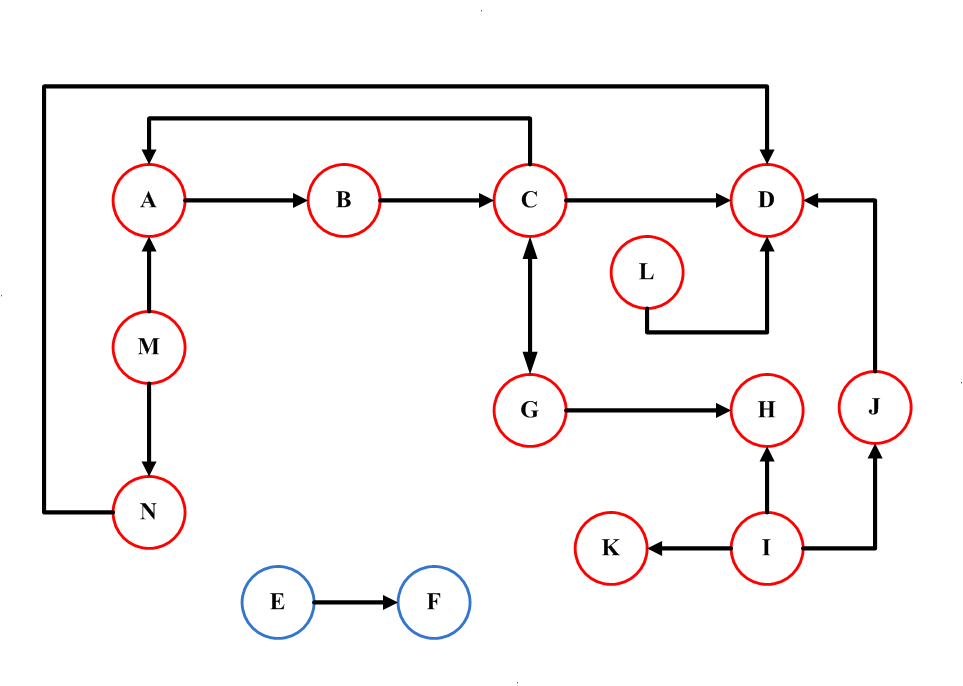
\includegraphics[scale=0.50]{assn01Q03}
\caption{Visual representation of the connecting nodes}
\end{figure}

\end{document}